
\def\freefont{} % 使用免费商业字体
\newcommand{\mytitleen}{Typesetting Tutorial for \LaTeX}
\newcommand{\mytitle}{\LaTeX 排版教程}
\newcommand{\myauthor}{兔子草}
\newcommand{\myquote}{\hfill ——排版,只需要一个浏览器\hspace{15mm}}
\def\version{1.0}

\ifdefined\freefont
    \usepackage{fontspec}
    \usepackage[fontset=none]{ctex}
    \setmainfont{EB Garamond 12 Regular}[Ligatures={Rare,Historic},Numbers=Lining,BoldFont=[EBGaramond08-Regular]]
    \setmonofont{Maple Mono Normal}

    \newfontfamily\ssfont{Vollkorn Medium Italic}
    \newfontfamily\chenfont{Vollkorn Italic}
    \newfontfamily\pagenfont{Vollkorn Italic}
    \newfontfamily\prenotefonten{EB Garamond 12 Regular}
    \newfontfamily\cpfont{Vollkorn}
    \newfontfamily\scfont{EB Garamond SmallCaps 12 Regular}

    \newfontfamily\mainreg{EB Garamond 12 Regular}[Numbers=Lining,Scale=1.2]
    \newfontfamily\mainsb{Vollkorn}[Numbers=Lining,Scale=1.15]
    \newfontfamily\mainb{Vollkorn Medium}[Scale=1.15,LetterSpace=-1]

    \newfontfamily\titlefonten{Allura}[LetterSpace=1]
    \newfontfamily\tempfont{Source Han Serif CN}

    \setCJKmainfont{Source Han Serif CN}[BoldFont=Source Han Serif CN SemiBold, ItalicFont=FZFangSong-Z02,BoldItalicFont=Source Han Serif CN Bold]
    \setCJKmonofont{FZHei-B01}

    \newCJKfontfamily\elsong{Source Han Serif CN ExtraLight}
    \newCJKfontfamily\lsong{Source Han Serif CN Light}
    \newCJKfontfamily\songti{Source Han Serif CN}
    \newCJKfontfamily\mediumsong{Source Han Serif CN Medium}
    \newCJKfontfamily\sbsong{Source Han Serif CN SemiBold}
    \newCJKfontfamily\bsong{Source Han Serif CN Bold}
    \newCJKfontfamily\hsong{Source Han Serif CN Heavy}

    \newCJKfontfamily\shusong{FZShuSong-Z01}[ItalicFont=FZKai-Z03] % 书宋
    \newCJKfontfamily\fangsong{FZFangSong-Z02} % 仿宋
    \newCJKfontfamily\heiti{FZHei-B01} % 黑体
    \newCJKfontfamily\kaiti{FZKai-Z03} % 楷体


    \newcommand{\titlefont}{\titlefonten\fangsong}
    \newcommand{\signfont}{\writing}

    \newcommand{\tocmain}{\bsong}
    \newcommand{\tocpart}{\sbsong\ssfont}
    \newcommand{\tocchapter}{\sbsong\chenfont}
    \newcommand{\tocchaplabel}{\itshape}
    \newcommand{\tocsection}{\songti}
    \newcommand{\tocsectlabel}{\scfont}
    \newcommand{\tocsubsection}{\tocsection}
    \newcommand{\tocsubsectlabel}{\tocsectlabel}
    \newcommand{\tocpage}{\pagenfont}

    \newcommand{\partfont}{\bsong\mainb}
    \newcommand{\chapterfont}{\bsong\mainb}
    \newcommand{\sectionfont}{\sbsong\mainsb}
    \newcommand{\subsectionfont}{\songti\mainreg}
    \newcommand{\pagenumberfont}{\tocpage}
    \newcommand{\headfont}{\kaiti\cpfont}
    \newcommand{\quotefont}{\itshape}
    \newcommand{\prenotefont}{\prenotefonten\sbsong}
    \newcommand{\writing}{\rmfamily\sbsong}
    \newcommand{\spellfont}{\quotefont}
    \newcommand{\dotfont}{\shusong}
\else
    \usepackage{ctex}
    \newcommand{\prenotefont}{\rmfamily}
    \newcommand{\titlefont}{}
    \newcommand{\signfont}{\ttfamily}
    \newcommand{\cpfont}{\ttfamily}

    \newcommand{\tocmain}{\bfseries}
    \newcommand{\tocpart}{\bfseries}
    \newcommand{\tocchapter}{\itshape}
    \newcommand{\tocchaplabel}{\itshape}
    \newcommand{\tocsection}{\rmfamily}
    \newcommand{\tocsectlabel}{\rmfamily}
    \newcommand{\tocsubsection}{\tocsection}
    \newcommand{\tocsubsectlabel}{\tocsectlabel}
    \newcommand{\tocpage}{\ttfamily}
    \newcommand{\ssfont}{\itshape}

    \newcommand{\partfont}{\bfseries\itshape}
    \newcommand{\chapterfont}{\bfseries}
    \newcommand{\sectionfont}{\bfseries}
    \newcommand{\subsectionfont}{\sffamily}
    \newcommand{\pagenumberfont}{\tocpage}
    \newcommand{\headfont}{\ttfamily}
    \newcommand{\quotefont}{\itshape}
    \newcommand{\writing}{\rmfamily\ttfamily}
    \newcommand{\spellfont}{\quotefont}
    \newcommand{\dotfont}{\rmfamily}
    \newcommand{\tempfont}{\rmfamily}
\fi

% % 字体配置
\ifdefined\freefont
    \usepackage{fontspec}
    \usepackage[fontset=none]{ctex}
    \setmainfont{EB Garamond 12 Regular}[Ligatures={Rare,Historic},Numbers=Lining,BoldFont=[EBGaramond08-Regular]]
    \setmonofont{Maple Mono Normal}

    \newfontfamily\ssfont{Vollkorn Medium Italic}
    \newfontfamily\chenfont{Vollkorn Italic}
    \newfontfamily\pagenfont{Vollkorn Italic}
    \newfontfamily\prenotefonten{EB Garamond 12 Regular}
    \newfontfamily\cpfont{Vollkorn}
    \newfontfamily\scfont{EB Garamond SmallCaps 12 Regular}

    \newfontfamily\mainreg{EB Garamond 12 Regular}[Numbers=Lining,Scale=1.2]
    \newfontfamily\mainsb{Vollkorn}[Numbers=Lining,Scale=1.15]
    \newfontfamily\mainb{Vollkorn Medium}[Scale=1.15,LetterSpace=-1]

    \newfontfamily\titlefonten{Allura}[LetterSpace=1]
    \newfontfamily\tempfont{Source Han Serif CN}

    \setCJKmainfont{Source Han Serif CN}[BoldFont=Source Han Serif CN SemiBold, ItalicFont=FZFangSong-Z02,BoldItalicFont=Source Han Serif CN Bold]
    \setCJKmonofont{FZHei-B01}

    \newCJKfontfamily\elsong{Source Han Serif CN ExtraLight}
    \newCJKfontfamily\lsong{Source Han Serif CN Light}
    \newCJKfontfamily\songti{Source Han Serif CN}
    \newCJKfontfamily\mediumsong{Source Han Serif CN Medium}
    \newCJKfontfamily\sbsong{Source Han Serif CN SemiBold}
    \newCJKfontfamily\bsong{Source Han Serif CN Bold}
    \newCJKfontfamily\hsong{Source Han Serif CN Heavy}

    \newCJKfontfamily\shusong{FZShuSong-Z01}[ItalicFont=FZKai-Z03] % 书宋
    \newCJKfontfamily\fangsong{FZFangSong-Z02} % 仿宋
    \newCJKfontfamily\heiti{FZHei-B01} % 黑体
    \newCJKfontfamily\kaiti{FZKai-Z03} % 楷体


    \newcommand{\titlefont}{\titlefonten\fangsong}
    \newcommand{\signfont}{\writing}

    \newcommand{\tocmain}{\bsong}
    \newcommand{\tocpart}{\sbsong\ssfont}
    \newcommand{\tocchapter}{\sbsong\chenfont}
    \newcommand{\tocchaplabel}{\itshape}
    \newcommand{\tocsection}{\songti}
    \newcommand{\tocsectlabel}{\scfont}
    \newcommand{\tocsubsection}{\tocsection}
    \newcommand{\tocsubsectlabel}{\tocsectlabel}
    \newcommand{\tocpage}{\pagenfont}

    \newcommand{\partfont}{\bsong\mainb}
    \newcommand{\chapterfont}{\bsong\mainb}
    \newcommand{\sectionfont}{\sbsong\mainsb}
    \newcommand{\subsectionfont}{\songti\mainreg}
    \newcommand{\pagenumberfont}{\tocpage}
    \newcommand{\headfont}{\kaiti\cpfont}
    \newcommand{\quotefont}{\itshape}
    \newcommand{\prenotefont}{\prenotefonten\sbsong}
    \newcommand{\writing}{\rmfamily\sbsong}
    \newcommand{\spellfont}{\quotefont}
    \newcommand{\dotfont}{\shusong}
\else
    \usepackage{ctex}
    \newcommand{\prenotefont}{\rmfamily}
    \newcommand{\titlefont}{}
    \newcommand{\signfont}{\ttfamily}
    \newcommand{\cpfont}{\ttfamily}

    \newcommand{\tocmain}{\bfseries}
    \newcommand{\tocpart}{\bfseries}
    \newcommand{\tocchapter}{\itshape}
    \newcommand{\tocchaplabel}{\itshape}
    \newcommand{\tocsection}{\rmfamily}
    \newcommand{\tocsectlabel}{\rmfamily}
    \newcommand{\tocsubsection}{\tocsection}
    \newcommand{\tocsubsectlabel}{\tocsectlabel}
    \newcommand{\tocpage}{\ttfamily}
    \newcommand{\ssfont}{\itshape}

    \newcommand{\partfont}{\bfseries\itshape}
    \newcommand{\chapterfont}{\bfseries}
    \newcommand{\sectionfont}{\bfseries}
    \newcommand{\subsectionfont}{\sffamily}
    \newcommand{\pagenumberfont}{\tocpage}
    \newcommand{\headfont}{\ttfamily}
    \newcommand{\quotefont}{\itshape}
    \newcommand{\writing}{\rmfamily\ttfamily}
    \newcommand{\spellfont}{\quotefont}
    \newcommand{\dotfont}{\rmfamily}
    \newcommand{\tempfont}{\rmfamily}
\fi


% 首段缩进
\usepackage{indentfirst}

% 启用并隐藏超链接
\usepackage{hyperref}
\hypersetup{hidelinks}

% 调整行距
\usepackage{setspace}
\newcommand{\mysetspacing}{
    \setstretch{1.618}
}
\mysetspacing

% 段距
\setlength{\parskip}{0pt}

% 页面配置
\usepackage{geometry}
% 主布局
\newlength{\pw}
\newlength{\ph}
% A5 148*210
\setlength{\pw}{148mm}
\setlength{\ph}{210mm}

\newlength{\bleedlen}
\setlength{\bleedlen}{0mm}

\newlength{\ptop}
\newlength{\pbottom}
\newlength{\pinner}
\newlength{\pouter}
\newlength{\phsep}
\newlength{\pfskip}

\setlength{\ptop}{21mm}
\setlength{\pbottom}{21mm}
\setlength{\pinner}{22mm}
\setlength{\pouter}{13.5mm}
\setlength{\phsep}{.8\baselineskip}
\setlength{\pfskip}{2.2\baselineskip}
\addtolength{\pfskip}{-1em}
% 目录页布局
\newcommand{\tocgeo}{}
% 图片页布局
\newcommand{\picgeo}{\newgeometry{top=\bleedlen,bottom=\bleedlen,inner=\bleedlen,outer=\bleedlen}}
% 图片页布局
\newcommand{\buindinpicgeo}{}

\ifdefined\bleed
    \addtolength{\bleedlen}{3mm}
    \addtolength{\pw}{\bleedlen}
    \addtolength{\pw}{\bleedlen}
    \addtolength{\ph}{\bleedlen}
    \addtolength{\ph}{\bleedlen}
    \addtolength{\ptop}{\bleedlen}
    \addtolength{\pbottom}{\bleedlen}
    \addtolength{\pinner}{\bleedlen}
    \addtolength{\pouter}{\bleedlen}
    \renewcommand{\tocgeo}{\newgeometry{left=30mm,right=30mm,top=\ptop,bottom=\pbottom}}
\else
    \renewcommand{\tocgeo}{\newgeometry{left=27mm,right=27mm,top=\ptop,bottom=\pbottom}}
\fi

\newcommand{\charcount}{32}
\newcommand{\linecount}{25}

\newlength{\theight}
\setlength{\theight}{\linecount\baselineskip}
\addtolength{\theight}{1em}
\addtolength{\theight}{-\baselineskip}

\geometry{
    paperwidth=\pw,
    paperheight=\ph,
    top=\ptop,
    outer=\pouter,
    % inner=\pinner,
    % bottom=\pbottom,
    textwidth=\charcount\ccwd,
    textheight=\theight,
    headsep=\phsep,
    footskip=\pfskip
}

% 空白页
\newcommand{\blankpage}{
    \newpage
    \makebox{}
    \thispagestyle{empty}
    \newpage
}

% 空白段
\newcommand{\blankpar}{
    ~\
}

% 目录
% 目录参数
\counterwithout{section}{chapter}
\counterwithout{subsection}{section}
% 目录格式
\usepackage{titletoc}
% 章节符号
\newcommand{\myss}{\ssfont\S}
% 目录标题
\renewcommand{\contentsname}{
    目\quad 录
}
% 目录内标题格式
\titlecontents{part}
[0em]
{\vspace{1em}\Large\tocpart}
{}
{}
{\hspace{4mm}\pagenumberfont\contentspage}[\vspace{0.5em}]

\titlecontents{chapter}
[6mm]
{\vspace{0.3em}\large\tocchapter}
{\makebox[10mm][l]{\myss\hspace{0.1em}\normalsize\uppercase\expandafter{\romannumeral\thecontentslabel}}}
{}
{\hspace{4mm}\tocpage\large\contentspage}[\vspace{0.3em}]

\titlecontents{section}
[12mm]
{\tocsection}
{\tocsectlabel Ch \hspace{0.1em}\makebox[1em][c]{\thecontentslabel}\hspace{1em}}{}
{\hspace{5mm}\tocpage\contentspage}[\vspace{0.1em}]

\makeatletter
% 页码宽度
\renewcommand{\contentspage}[1][\thecontentspage]{\hb@xt@\@pnumwidth{#1\hfil}}
\renewcommand{\@pnumwidth}{9mm}
% 每章重置尾注编号
\@addtoreset{endnote}{chapter}  % Reset endnote numbering every new chapter
\@addtoreset{subsection}{section} % Reset subsection numbering every new section
\@addtoreset{section}{chapter} % Reset section numbering every new chapter
\@addtoreset{chapter}{part}  % Reset chapter numbering every new part
\makeatother
% 每页重置脚注编号
\usepackage{footnpag}

% 正文标题格式
\usepackage{titlesec}

\titleformat{\part}[display]{\centering\huge\partfont}{\thepart}{1.5pc}{\thispagestyle{empty}}
\titlespacing{\part}{0em}{.3\textheight}{0em}

\titleformat{\chapter}{\centering\Large\chapterfont}{}{0em}{}
\titlespacing{\chapter}{0em}{.5\baselineskip}{2\baselineskip}

\titleformat{\section}{\sectionfont}{Chapter~\thesection}{1em}{}
\titlespacing{\section}{2em}{1.4\baselineskip plus 2pt minus 2pt}{.5\baselineskip plus 2pt minus 2pt}

\titleformat{\subsection}{\subsectionfont}{0\thesubsection}{1em}{}
\titlespacing{\subsection}{2em}{.5\baselineskip plus 2pt minus 2pt}{.5\baselineskip plus 2pt minus 2pt}

\newcommand{\parttitle}{部名}

\usepackage{fancyhdr}
% 章节标记不出现chapter和序号
\renewcommand{\chaptermark}[1]{\markboth{\MakeUppercase{#1}}{}}
\renewcommand{\sectionmark}[1]{\markright{#1}}
% 去除页眉横线
\renewcommand{\headrulewidth}{0pt}
% 页脚溢出一点
\fancyfootoffset[RO,LE]{1.5em}
\fancypagestyle{mystyle}{
    \fancyhf{}
    \fancyhead[CE]{\headfont\mytitle}
    \fancyhead[CO]{\headfont\parttitle}
    \fancyfoot[CO]{\hfill\headfont\leftmark\qquad\rule[-4pt]{0.3pt}{20pt}\hspace{1.5em}}
    \fancyfoot[RO]{\pagenumberfont\thepage}
    \fancyfoot[LE]{\pagenumberfont\thepage}
    \fancyfoot[CE]{\hspace{1.5em}\rule[-4pt]{0.3pt}{20pt}\qquad\headfont\parttitle\hfill}
}
\fancypagestyle{plain}{
    \fancyhf{}
    \fancyfoot[CO]{\hfill\headfont\leftmark\qquad\rule[-4pt]{0.3pt}{20pt}\hspace{1.5em}}
    \fancyfoot[RO]{\pagenumberfont\thepage}
    \fancyfoot[LE]{\pagenumberfont\thepage}
    \fancyfoot[CE]{\hspace{1.5em}\rule[-4pt]{0.3pt}{20pt}\qquad\headfont\parttitle\hfill}
}
\usepackage{emptypage}

% 尾注
\usepackage{endnotes}
\renewcommand{\notesname}{注:}
\renewcommand{\enoteheading}{\section*{\notesname}\mbox{}\par\vskip-\baselineskip}
\renewcommand{\theendnote}{\roman{endnote}}

% 以下为非通用内容

% 故事完
\newcommand{\storyend}[1][完]{
    \vspace{1.5\baselineskip}

    \blankpar

    \hfill \textbf{#1} \hspace{5em}

    \vspace{2\baselineskip}

    \vfill
}

\usepackage{changepage}
\renewenvironment{quotation}{
    \begin{adjustwidth}{2em}{2em}
        \quotefont
        }{
    \end{adjustwidth}
    \vspace{.5\baselineskip plus .5\baselineskip}
}
\renewenvironment{quote}{
    \vspace{0pt plus .3\baselineskip}

    \begin{adjustwidth}{2em}{2em}
        \quotefont}{
    \end{adjustwidth}

    \vspace{.3\baselineskip}
}


% 设置署名
\newcommand{\signature}{
    \vfill
    \setstretch{1.5}

    \begin{figure}[h]
        \hfill\includegraphics[width=2.8em]{headshot.png}\hspace{5.1em}
    \end{figure}

    \vspace{-1.5em}

    \hfill {\subsectionfont by\myauthor}\hspace{5em}

    \hfill {\subsectionfont \number\year.\number\month.\number\day} \hspace{4.8em}

    \vspace{2cm}
}

% 特殊符号和字体
\newcommand{\splitdot}{\dotfont ·}

\newcommand{\spell}[1]{{\spellfont #1}}

\newcommand{\tempsymbol}{{\tempfont℃}}

\newcommand{\chsline}{\makebox[2em]{——}}

% 章前注
\newcommand{\prenotes}[1]{
    \vspace{2em}
    {\prenotefont #1}
    % #1
    \vspace{0.5em}
}
% 章前注的参数
\newlength{\chapterblank}
\setlength{\chapterblank}{3cm}
\newlength{\prenoteblank}
\setlength{\prenoteblank}{3em}
\newcommand{\doublelinechapter}{{\huge\vspace{-\baselineskip}}}

% 扉页
\newcommand{\mytitlepage}{
    \null
    \vfill
    \thispagestyle{empty}

    \begin{center}
        \Huge

        \titlefont

        {\mytitleen}

        \vspace{2mm}

        {\mytitle}

        \Large

        \vspace{60mm}

        {\cpfont\mycp}

        \vspace{2mm}

        {\signfont BY \myauthor}
    \end{center}

    \vfill

    \clearpage
}

% 尾页
\newcommand{\myendpage}{
    \newpage
    \ifodd\thepage
        \blankpage
    \fi

    \newpage

    \thispagestyle{empty}

    \

    \vfill

    \begin{minipage}{50mm}

        模板制作:兔子草

    \end{minipage}
    \vspace{5mm}
}

% 插入图片
\usepackage{graphicx}

% 让脚注不影响上文的行距
\usepackage[bottom]{footmisc}
% 脚注上方高度
\setlength{\footnotesep}{8pt}
% 脚注上方横线
\renewcommand{\footnoterule}{
    \kern -2pt
    \hrule width .25\textwidth height 0.5pt
    \kern 1.5pt
}

% section上方弹性换页
\usepackage{needspace}
\AddToHook{cmd/section/before}{\needspace{3\baselineskip}}

\let\origpart\part
\renewcommand*{\part}[2][]{
    \ifx\\#1\\% optional argument not present?
    \origpart{#2}
        \renewcommand*\parttitle{#2}
    \else
    \origpart[#1]{#2}
        \renewcommand*\parttitle{#1}
    \fi
    \mysetspacing
}


\usepackage{setspace}

% 这部分设定纯为教程服务 
\usepackage{xcolor}
\definecolor{gray}{RGB}{68,71,90}
\definecolor{grayblue}{RGB}{98,144,164}
\definecolor{cyan}{RGB}{139, 233, 253}
\definecolor{green}{RGB}{80, 250, 123}
\definecolor{orange}{RGB}{255, 184, 108}
\definecolor{pink}{RGB}{255, 121, 198}
\definecolor{purple}{RGB}{189, 147, 249}
\definecolor{red}{RGB}{255, 85, 85}
\definecolor{yellow}{RGB}{241, 250, 140}
\definecolor{myblack}{RGB}{32, 34, 39}
\definecolor{darkgreen}{RGB}{31,138,35}
\usepackage{hyperref}
\hypersetup{colorlinks,linkcolor=black,urlcolor=darkgreen}
\usepackage{metalogo}
\usepackage{enumitem}
\usepackage[normalem]{ulem}
\usepackage{listings}
\renewcommand{\lstlistingname}{代码}
\renewcommand{\lstlistlistingname}{代码}
\lstset{
    flexiblecolumns,
    numbers=left,
    numberstyle=\footnotesize\color{gray},
    frame=leftline,
    showspaces=false,
    linewidth=\linewidth,
    xleftmargin=2\ccwd,
    breaklines=true,
    columns=fixed,
    basicstyle=\small\ttfamily,
    captionpos=b,
}
\lstdefinestyle{TeX}{
    language=TeX,
    morekeywords={usepackage,begin,newcommand,renewcommand,counterwithout,setcounter,addcounter,part,chapter,section,clearpage,newpage,cleardoublepage,thepage,setlength,addtolength,newlength,ctexset,plus,minus,makeatletter,makeatother,patchcmd,@addtoreset,addcontentsline},
    emph={documentclass,document,setmainfont,newfontfamily,BoldFont,ItalicFont,setCJKmainfont,newCJKfontfamily,geometry,newgeometry,restoregeometry,titleformat,titlespacing,blankpage,singlespacing,onehalfspacing,doublespacing,setstretch,pagestyle,thispagestyle,punctstyle,roman,titlecontents,vspace,hspace,makebox,mbox,@pnumwidth,startcontents,stopcontents,printcontents,hypersetup,fancypagestyle,fancyhf,fancyhead,fancyfoot,markboth,markright,fancyhfoffset,fancyheadoffset,fancyfootoffset,includegraphics,figure,caption,captionsetup,includepdf,subfile},
    basicstyle=\small\ttfamily\color{myblack},
    identifierstyle=\color{purple},
    keywordstyle=\color{pink},
    emphstyle=\color{orange},
    stringstyle=\color{yellow},
    commentstyle=\color{grayblue},
}
\usepackage{makecell}
\newcommand{\emoji}[1]{{\fontspec{Symbola}\symbol{#1}}}
\newcommand{\checkmark}{
    \makebox[1\ccwd]{
        \fboxsep1.5pt
        \colorbox{green}{\emoji{"2714}}
    }
}
\usepackage{longtable}
\newenvironment{tightitem}
{\begin{itemize}[topsep=0pt,partopsep=0pt,itemsep=0pt,parsep=0pt,leftmargin=3\ccwd,labelwidth=1.5\ccwd,labelsep=.5\ccwd]}
        {\end{itemize}}

\newenvironment{tightenum}
{\begin{enumerate}[topsep=0pt,partopsep=0pt,itemsep=0pt,parsep=0pt,leftmargin=3\ccwd,labelwidth=1.5\ccwd,labelsep=.5\ccwd]}
        {\end{enumerate}}

\newcommand{\testtext}{

    Hal低低地笑了:“我希望你把蝙蝠车留给Tim,然后回家。……他说愿意替你7个小时的班,让你休息一下。”}
\usepackage{float}
\usepackage{fancyhdr}
\renewcommand{\chaptermark}[1]{\markboth{\MakeUppercase{#1}}{}}
\renewcommand{\sectionmark}[1]{\markright{#1}}
% 去除页眉横线
\renewcommand{\headrulewidth}{0pt}
% 页脚溢出一点
\fancyfootoffset[RO,LE]{1.5em}
\fancypagestyle{mystyle}{
    \fancyhf{}
    \fancyhead[CE]{\headfont\mytitle}
    \fancyhead[CO]{\headfont\uppercase\expandafter{\romannumeral\thechapter}\quad\leftmark}
    \fancyfoot[CO]{\hfill\headfont BY \myauthor\qquad\rule[-4pt]{0.3pt}{20pt}\hspace{1.5em}}
    \fancyfoot[RO]{\pagenumberfont\thepage}
    \fancyfoot[LE]{\pagenumberfont\thepage}
    \fancyfoot[CE]{\hspace{1.5em}\rule[-4pt]{0.3pt}{20pt}\qquad\headfont\uppercase\expandafter{\romannumeral\thechapter}\hfill}
}
\fancypagestyle{plain}{
    \fancyhf{}
    \fancyfoot[CO]{\hfill\headfont BY \myauthor\qquad\rule[-4pt]{0.3pt}{20pt}\hspace{1.5em}}
    \fancyfoot[RO]{\pagenumberfont\thepage}
    \fancyfoot[LE]{\pagenumberfont\thepage}
    \fancyfoot[CE]{\hspace{1.5em}\rule[-4pt]{0.3pt}{20pt}\qquad\headfont\uppercase\expandafter{\romannumeral\thechapter}\hfill}
}

\newlength{\ptop}
\newlength{\pbottom}
\newlength{\pinner}
\newlength{\pouter}
\newlength{\phsep}
\newlength{\pfskip}

\setlength{\ptop}{21mm}
\setlength{\pbottom}{21mm}
\setlength{\pinner}{14mm}
\setlength{\pouter}{13.5mm}
\setlength{\phsep}{.8\baselineskip}
\setlength{\pfskip}{2.2\baselineskip}
\addtolength{\pfskip}{-1em}

\newcommand{\charcount}{40}
\newcommand{\linecount}{41}

\newlength{\theight}
\setlength{\theight}{\linecount\baselineskip}
\addtolength{\theight}{1em}
\addtolength{\theight}{-\baselineskip}

\usepackage{geometry}
\geometry{
    paperwidth=6.625in,
    paperheight=10.25in,
    top=\ptop,
    inner=\pinner,
    % outer=\pouter,
    % bottom=\pbottom,
    textwidth=\charcount\ccwd,
    textheight=\theight,
    headsep=\phsep,
    footskip=\pfskip,
}

\counterwithout{section}{chapter}
\counterwithout{subsection}{section}
\makeatletter
\@addtoreset{section}{chapter}
\@addtoreset{subsection}{section}
\makeatother

\usepackage{titletoc}
\usepackage{titlesec}
\renewcommand{\contentsname}{目\quad 录}

\titlecontents{chapter}
[4mm]
{\vspace{0.3em}\large\tocchapter}
{\makebox[10mm][l]{\normalsize\uppercase\expandafter{\romannumeral\thecontentslabel}}}
{}
{\hfill\tocpage\large\contentspage}[\vspace{0.3em}]

\renewcommand{\tocsectlabel}{\fontspec{EB Garamond SmallCaps 12 Regular}[Numbers=Lining]}
\renewcommand{\sectionfont}{\tocsectlabel\sbsong}
\renewcommand{\subsectionfont}{\tocsubsection\songti}
\renewcommand{\tocsubsectlabel}{\subsectionfont}
\titlecontents{section}
[8mm]
{\tocsection}
{\tocsectlabel \S \hspace{0.1em}\makebox[1.2em][c]{\thecontentslabel}\hspace{1em}\sectionfont}{}
{\dotfill\tocpage\contentspage}

\titlecontents{subsection}
[16mm]
{\tocsubsection}
{\small\tocsubsectlabel\hspace{0.2em}\makebox[1em][c]{\expandafter{\romannumeral\thecontentslabel}}\hspace{0.8em}}{}
{\dotfill\small\tocpage\contentspage}{}

\titleformat{\chapter}{\centering\Large\chapterfont}{\uppercase\expandafter{\romannumeral\thechapter}}{1em}{}
\titlespacing{\chapter}{0em}{.5\baselineskip}{2\baselineskip}
\titleformat{\section}{\sectionfont}{\S~\thesection}{1em}{}
\titlespacing{\section}{2em}{1.4\baselineskip plus 2pt minus 2pt}{.5\baselineskip plus 2pt minus 2pt}
\titleformat{\subsection}{\subsectionfont}{\expandafter{\romannumeral\thesubsection}}{1em}{}
\titlespacing{\subsection}{2em}{.5\baselineskip plus 2pt minus 2pt}{.5\baselineskip plus 2pt minus 2pt}

\newcommand{\jumpto}[2]{\href{#1}{#2\footnote{#1}}}

\newcommand{\signature}{
    \vspace{2\baselineskip}
    \hfill\begin{minipage}[b]{6em}
        \begin{center}
            \includegraphics[width=2.8em]{../headshot.png}\hspace{5.1em}
            \subsectionfont
            by\myauthor

            \emoji{"1F427} 3440950898
        \end{center}
    \end{minipage}\hspace{4em}

    \vspace{2\baselineskip}
}

\newfontfamily\bcfont{BlackChancery}
\renewcommand{\titlefont}{\bcfont\bsong}
\newcommand{\mytitlepage}{
    \null
    \vspace{.18\textheight}
    \thispagestyle{empty}

    \begin{center}
        \Huge

        \titlefont

        {\mytitleen}

        \vspace{2mm}

        {\mytitle}

        \vspace{2mm}

        {\large\fangsong\myquote}

        \vspace{.32\textheight}

        \Large

        {\signfont BY \myauthor}

        {\large\signfont v\version}
    \end{center}

    \clearpage
}

\usepackage{changepage}

\newcommand{\blankpar}{
    ~\
}

\usepackage{indentfirst}

\usepackage{footnpag}

\usepackage{emptypage}

\usepackage{multicol}

% \usepackage{mathfont}

% \mathfont[greeklower]{EB Garamond 12 Italic}

\newcommand{\myendpage}{
    \clearpage
    \ifodd\thepage
    \else
        \mbox{}
        \thispagestyle{empty}
        \clearpage
    \fi
}
